\documentclass[12pt]{article}

\usepackage[a4paper,left=25mm,right=25mm,top=35mm,bottom=25mm]{geometry}
\usepackage{ngerman}
\usepackage{parskip}
\usepackage{times}
\usepackage{graphicx}
\usepackage{listings}
\usepackage{fancyhdr}
\usepackage{float}
\usepackage{amsmath}

\setlength{\headheight}{15.2pt}
\pagestyle{fancy}

\lhead{Bildverarbeitung und Mustererkennung\\Praktikum Blatt 7}
\rhead{Patrick Hüntelmann\\03.06.2022}

\lstset{
  basicstyle=\ttfamily,
  breakatwhitespace=false,         % sets if automatic breaks should only happen at whitespace
  breaklines=true,                 % sets automatic line breaking
  captionpos=b,                    % sets the caption-position to bottom
  deletekeywords={...},            % if you want to delete keywords from the given language
  escapeinside={\%*}{*)},          % if you want to add LaTeX within your code
  extendedchars=true,              % lets you use non-ASCII characters; for 8-bits encodings only, does not work with UTF-8
  frame=single,	                   % adds a frame around the code
  keepspaces=true,                 % keeps spaces in text, useful for keeping indentation of code (possibly needs columns=flexible)
  language=python,                 % the language of the code
  showstringspaces=false,          % underline spaces within strings only
  showtabs=false,                  % show tabs within strings adding particular underscores
  tabsize=2,	                   % sets default tabsize to 2 spaces
}

\begin{document}

\pagenumbering{arabic}

\section*{Aufgabe 7}
\subsection*{Teil 1. Template Matching}
\subsubsection*{a) Ähnlichkeitsmaße}
Das Ähnlichkeitsmaß \textit{sum of squared differences (SSD)} ist in der Funktion \textbf{ssd} (main.py Zeile 15) implementiert. Hier wird aus dem Referenzausschnitt und dem Templatebild ein Differenzbild erzeugt. Dieses Differenzbild wird anschließend quadriert und summiert.
Der \textit{Korrelationskoeffizient (COR)} ist in der Funktion \textbf{cor} (main.py Zeile 20) implementiert. Diese Funktion verteilt die Werte des Referenzausschnittes und dem Templatebild neu, anschließend teilt sie das Produkt aus den neuverteilten Bildern durch ein Produkt aus der Wurzel der Summe des quadrierten Bildes.

\subsubsection*{b) Suchstrategie}
Die Suchstrategie ist in der Funktion \textbf{aufgabe\_1} (main.py Zeile 36) implementiert. Diese Funktion teilt das Referenzbild in zum Template passende Ausschnitte ein und berechnet für jeden möglichen Ausschnitt die Ähnlichkeitsmaße \textit{SSD} und \textit{COR} und speichert diese in einem Bild ab.
Anschließend holt sich die Funktion zunächst den Index des Minima in dem \textit{SSD} Bild und zeichnet auf dem Ausgangsbild ein Rechteckt an diesem Index in der Größe des Templates und stellt dieses Ergebnisbild dar.
Aus dem \textit{COR} Bild wird der Index des Maximas gesucht. An dieser Stelle wird ebenfalls ein Rechteck gezeichnet und dieses dargestellt.

\newpage

\subsubsection*{Ergebnisbilder}
\begin{figure}[H]
  \centering
  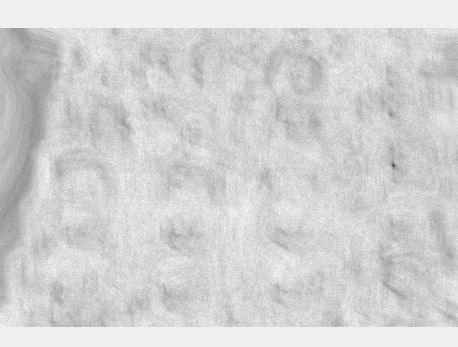
\includegraphics[width=0.7\textwidth, keepaspectratio]{ssd_values.png}\\
  \textit{SSD} Werte
\end{figure}
\begin{figure}[H]
  \centering
  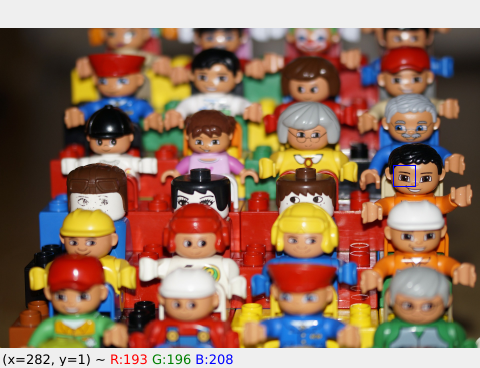
\includegraphics[width=0.7\textwidth, keepaspectratio]{ssd_match.png}\\
  \textit{SSD} Tiefpunkt
\end{figure}
\begin{figure}[H]
  \centering
  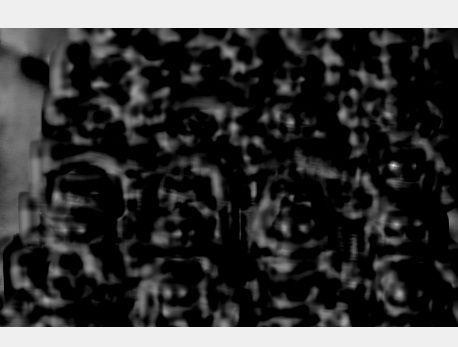
\includegraphics[width=0.7\textwidth, keepaspectratio]{cor_values.png}\\
  \textit{COR} Werte
\end{figure}
\begin{figure}[H]
  \centering
  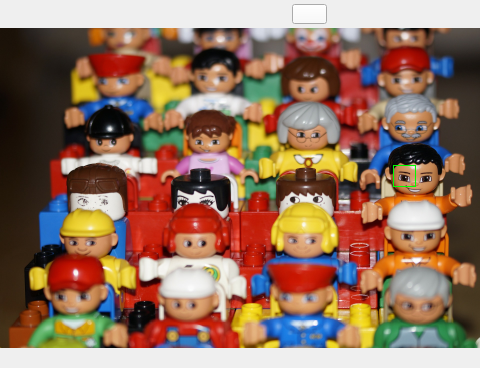
\includegraphics[width=0.7\textwidth, keepaspectratio]{cor_match.png}\\
  \textit{COR} Hochpunkt
\end{figure}

\newpage

\subsection*{Teil 2. Harris Corner Detector}
Der Harris Corner Detector ist in der Funktion \textbf{harris\_corner\_detector} (main.py Zeile 123) implementiert. Innerhalb dieser Funktion wird zunächst der Strukturtensor mit der Funktion \textbf{calculate\_structure\_tensor} (main.py Zeile 93) erzeugt. Diese Funktion erzeugt einen Gradienten des Bildes in x- und y-Richtung. Anschließend werden aus den Gradienten in x- und y-Richtung mögliche Produkte gebildet und diese mit einem Gaußfilter geglättet. Danach werden die Ergebnisse in einem Tupel zurückgegeben.
Nachdem der Strukturtensor erzeugt wurde wird mit der Funktion \textbf{calculate\_corner\_response\_function} (main.py Zeile 109) die Corner Response Funktion gebildet. Hierzu wird aus den Werten des Strukturtensors die Determinante und der Trace-Wert errechnet und auss diesen Werten die Corner Response Funktion.
Nachdem die Corner Response Funktion gebildet ist wird darauf ein Thresholding ausgeführt und anschließend eine Non-Maxima-Suppression. Hierbei wird das Maximum in der Funktion gesucht, an entsprechender Stelle im Ergebnisbild eine Markierung gezeichnet und der Wert auf 0 gesetzt, dann werden alle Werte mit einem euklidischen Abstand von $10$ ebenfalls auf 0 gesetzt. Dies wird solange wiederholt bis alle Werte auf 0 sind. 

\subsubsection*{Ergebnisbilder}
\begin{figure}[H]
  \centering
  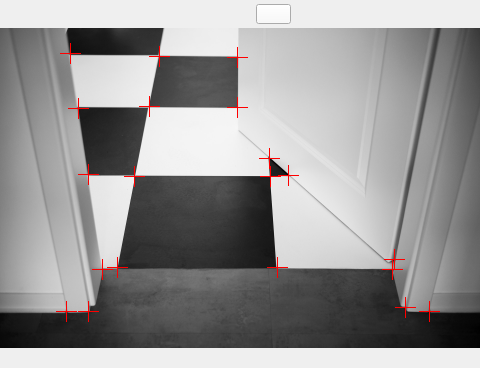
\includegraphics[width=0.8\textwidth, keepaspectratio]{harris_corner_detektor.png}\\
  Bild mit markierten Eckpunkten
\end{figure}

\end{document}
